\documentclass[UTF8]{beamer}
\usefonttheme[onlymath]{serif}

\usepackage[english]{babel}
\usepackage[utf8]{inputenc}
\usepackage[T1]{fontenc}
\usepackage{fixltx2e}
\usepackage{graphicx}
\usepackage{caption}
\usepackage[labelformat=simple, skip=10pt]{subcaption}
\usepackage{grffile}
\usepackage{longtable}
\usepackage{wrapfig}
\usepackage{rotating}
\usepackage[normalem]{ulem}
\usepackage{amsmath}
\usepackage{textcomp}
\usepackage{amssymb}
\usepackage{capt-of}
\usepackage{hyperref}
\usepackage{biblatex}
\usepackage{algorithm,algorithmic}
\usepackage{ctex}

\usetheme[sidebar]{XDUstyle}

\bibliographystyle{XDUbibunsrt}
\bibliography{ThesisFiles/RefFile}%在正文中必须引用,才能显示对应的参考文献

\title{机动车车牌的实时检测与识别系统}
\author[王昌旭]{王昌旭}
\institute[西安电子科技大学\\计算机学院]{西安电子科技大学计算机学院2012级本科生}
\date{\today}

\begin{document}

{ \xdbg
\begin{frame}[plain, noframenumbering]
  \titlepage
\end{frame}
}

\begin{frame}[t, allowframebreaks]
  \frametitle{目录}
  \tableofcontents
\end{frame}

\part{引言}

\section{研究意义}
\begin{frame}
  \frametitle{研究意义}
  机动车车牌识别有着十分广泛的的应用:

  \begin{itemize}
    \item 停车场智能管理
    \item 停车场自动找车系统
    \item 电子警察
    \item 无人驾驶汽车
  \end{itemize} 
\end{frame}

\begin{frame}
  \frametitle{研究意义}
  \begin{figure}[ht]
    \centering
    \subcaptionbox{校门口的停车场门禁系统}
    {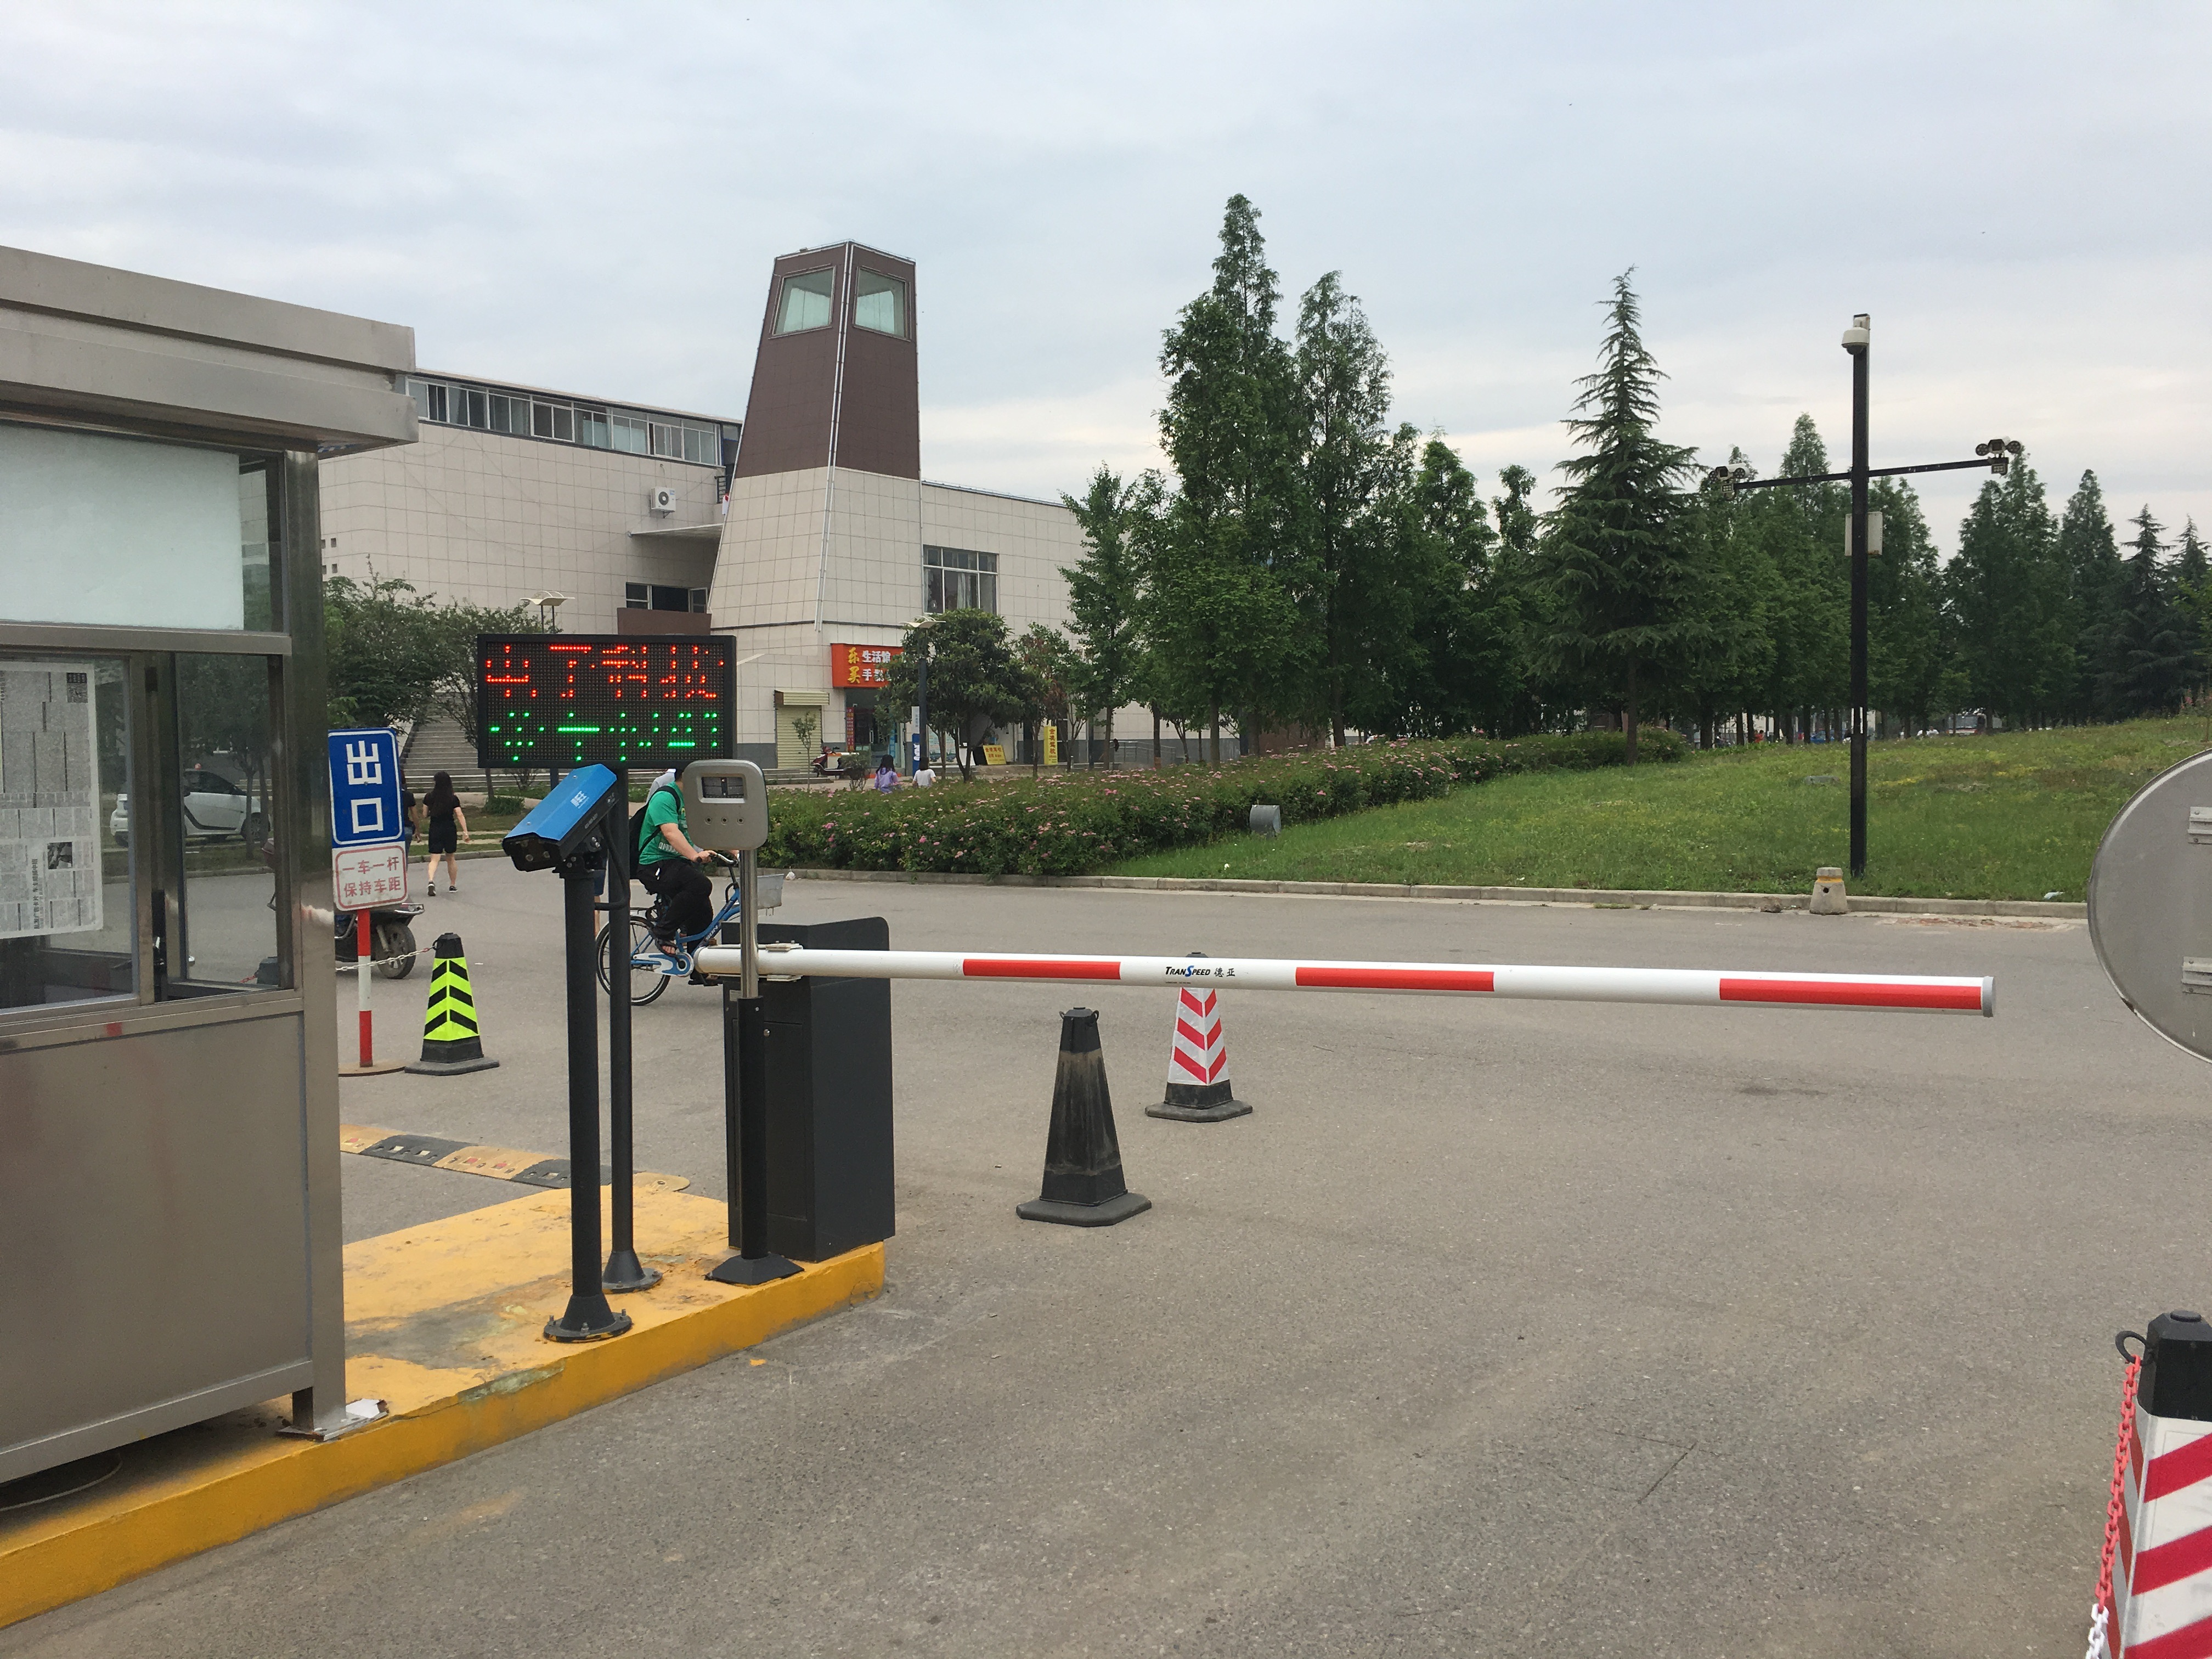
\includegraphics[width=0.45\linewidth]{./Figure/ParkingSystem.jpg}}
    \subcaptionbox{Google 的无人驾驶汽车}
    {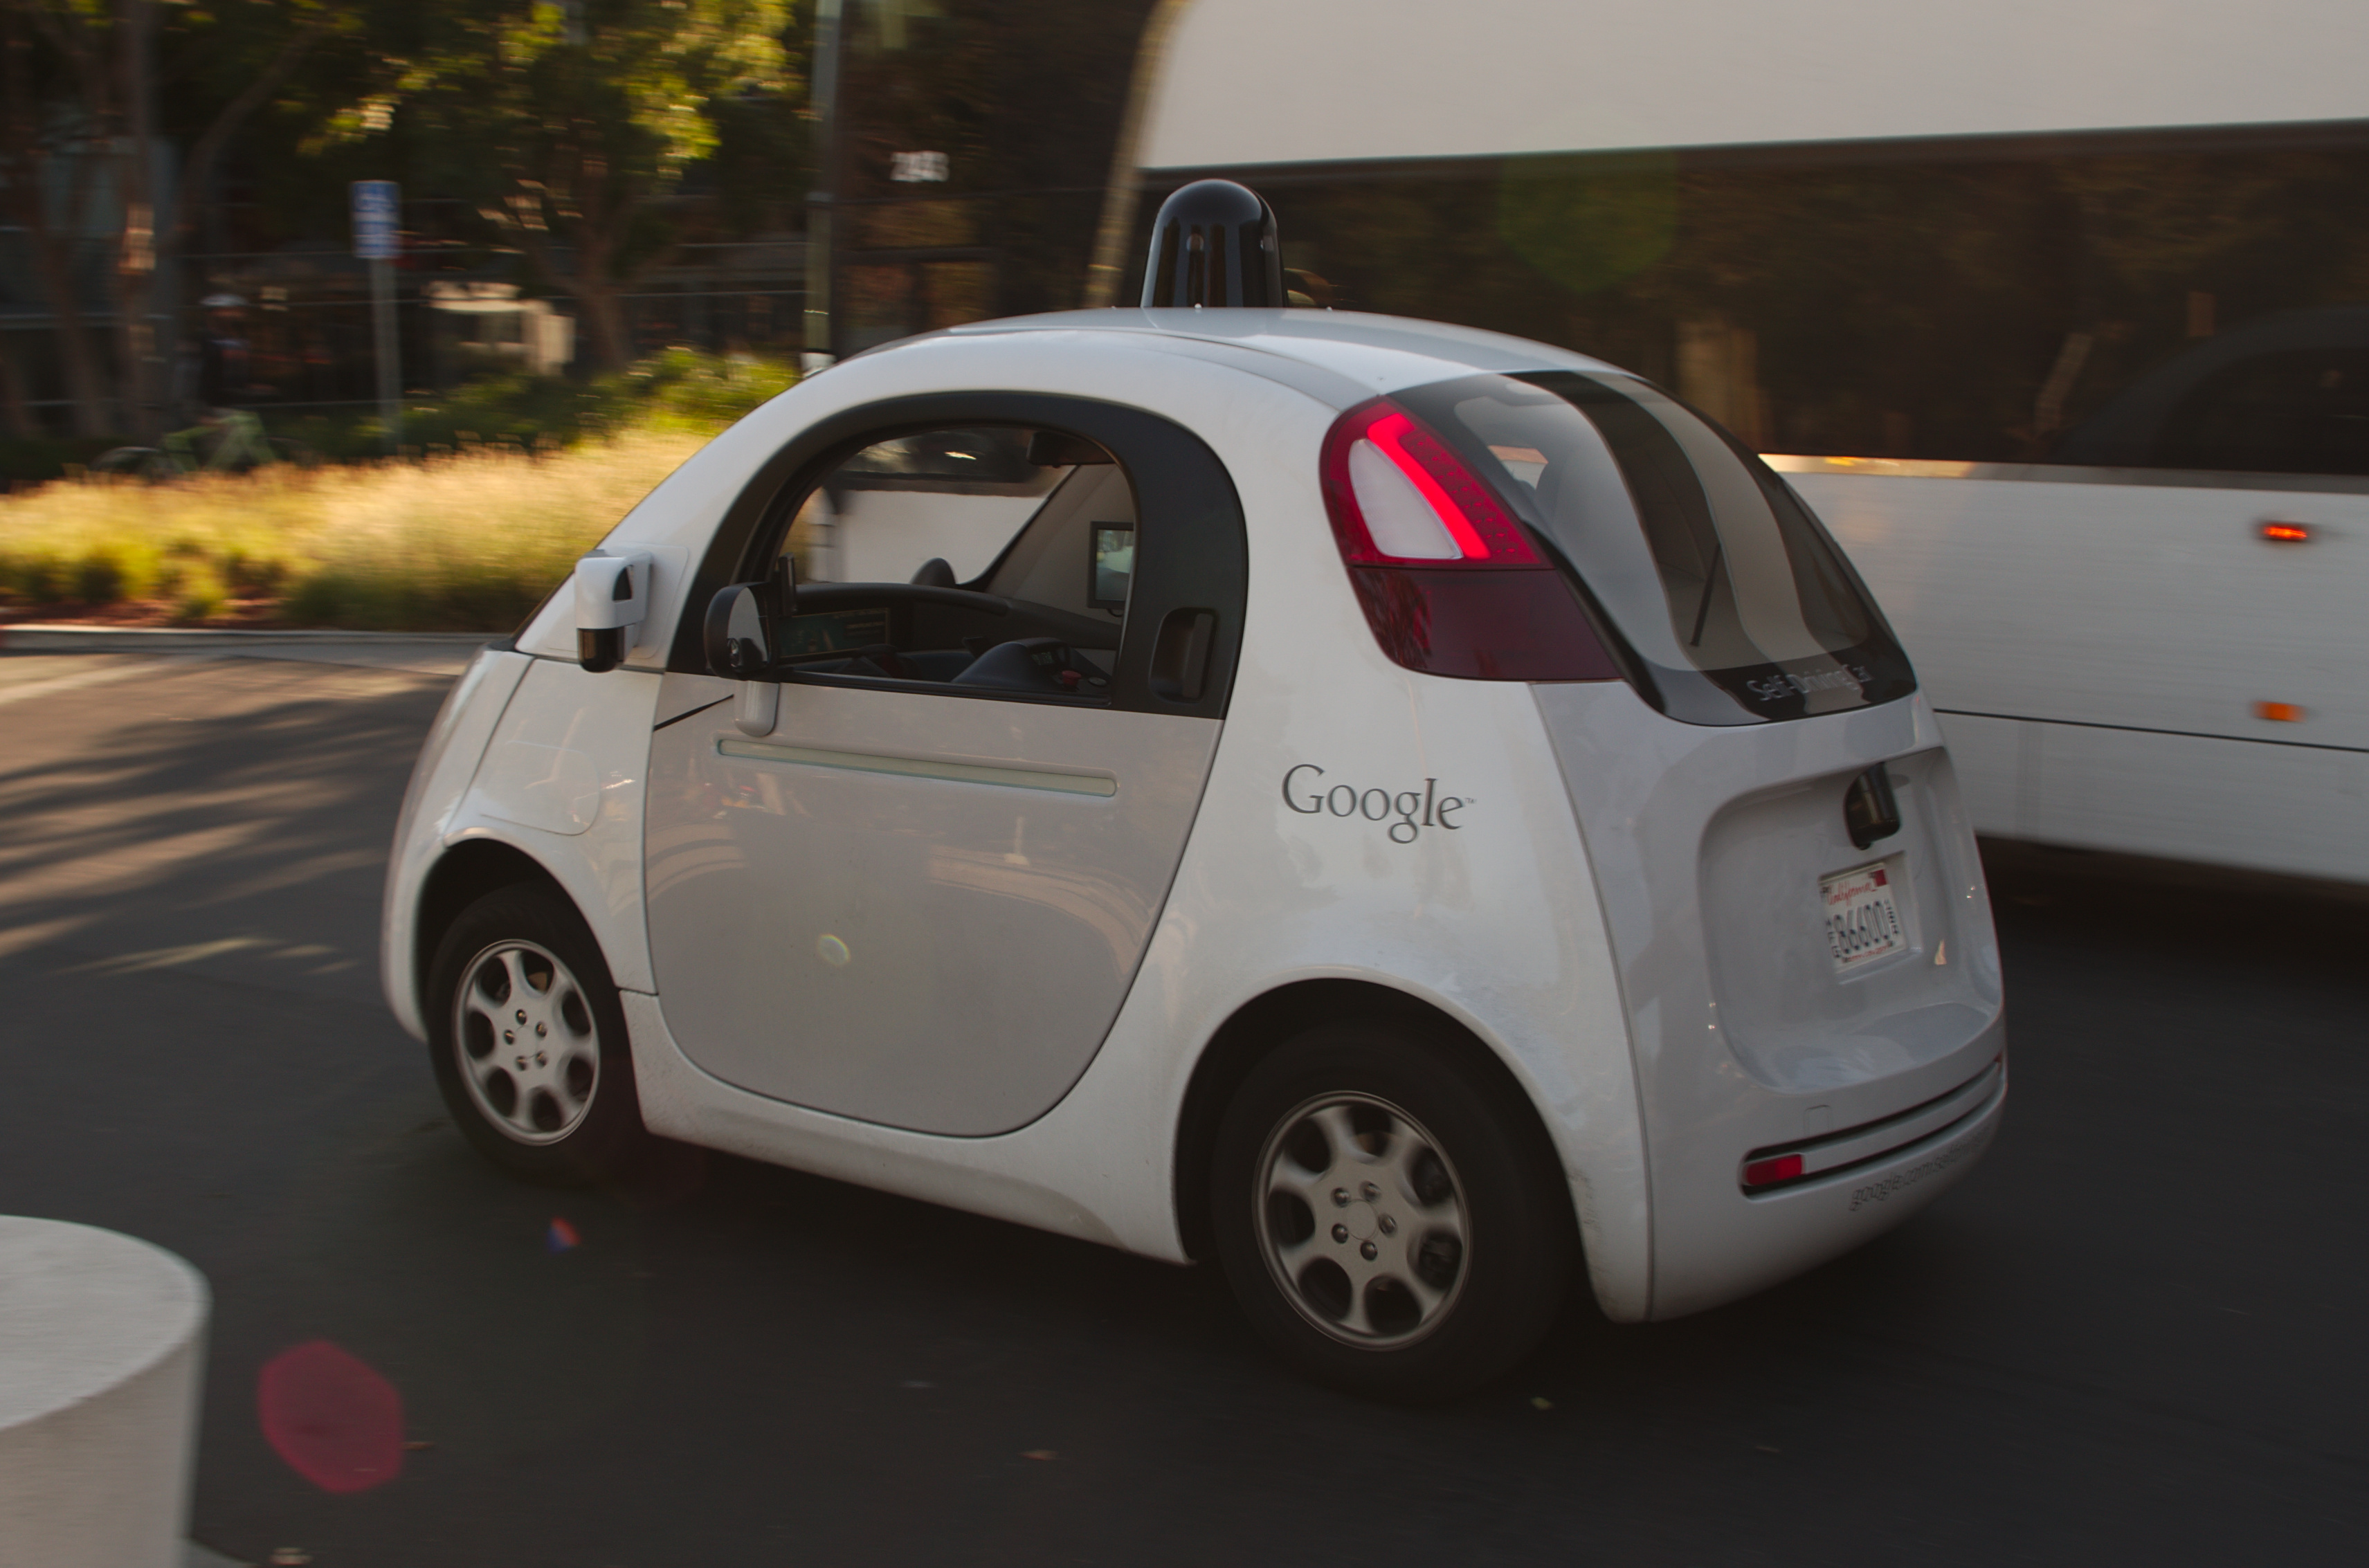
\includegraphics[width=0.45\linewidth]{./Figure/GoogleSelfDrivingCar.jpg}}
    \caption{车牌识别应用举例}
  \end{figure}
\end{frame}

\section{传统方法 VS 深度学习}

\begin{frame}
  \frametitle{传统方法 = 手工特征 + 模型}

  \textcolor{red}{\paragraph{优点}}
  \begin{itemize}
    \item 速度快,易于实现
    \item 便于进行理论分析   
  \end{itemize}

  \textcolor{red}{\paragraph{缺点}}
  \begin{itemize}
    \item 依赖大量先验知识及特征工程
    \item 对系统设计者要求高
    \item 对复杂任务效果不佳
  \end{itemize}
\end{frame}

\begin{frame}
  \frametitle{深度学习 = 数据 + 神经网络}

  \textcolor{red}{\paragraph{优点}}
  \begin{itemize}
    \item 人工干预少
    \item 对于复杂任务效果好
  \end{itemize}

  \textcolor{red}{\paragraph{缺点}}
  \begin{itemize}
    \item 对数据的数量和质量要求高
    \item 计算量大,速度慢
    \item 神经网络为黑箱系统,难以进行有效的数学分析
  \end{itemize}
\end{frame}

\begin{frame}
  \frametitle{CNN的结构}

  \begin{figure}[ht]
    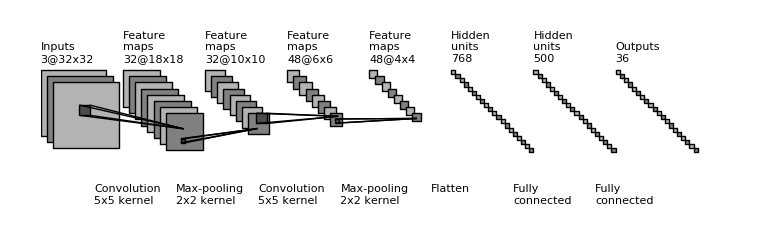
\includegraphics[width=1.0\linewidth]{./Figure/RecognitionAlnum.png}
    \caption{一个CNN模型示例}
  \end{figure}
\end{frame}
  
\section{车牌识别系统结构}

\begin{frame}
  \frametitle{车牌识别系统结构图}
  \begin{figure}[ht]
    \centering
    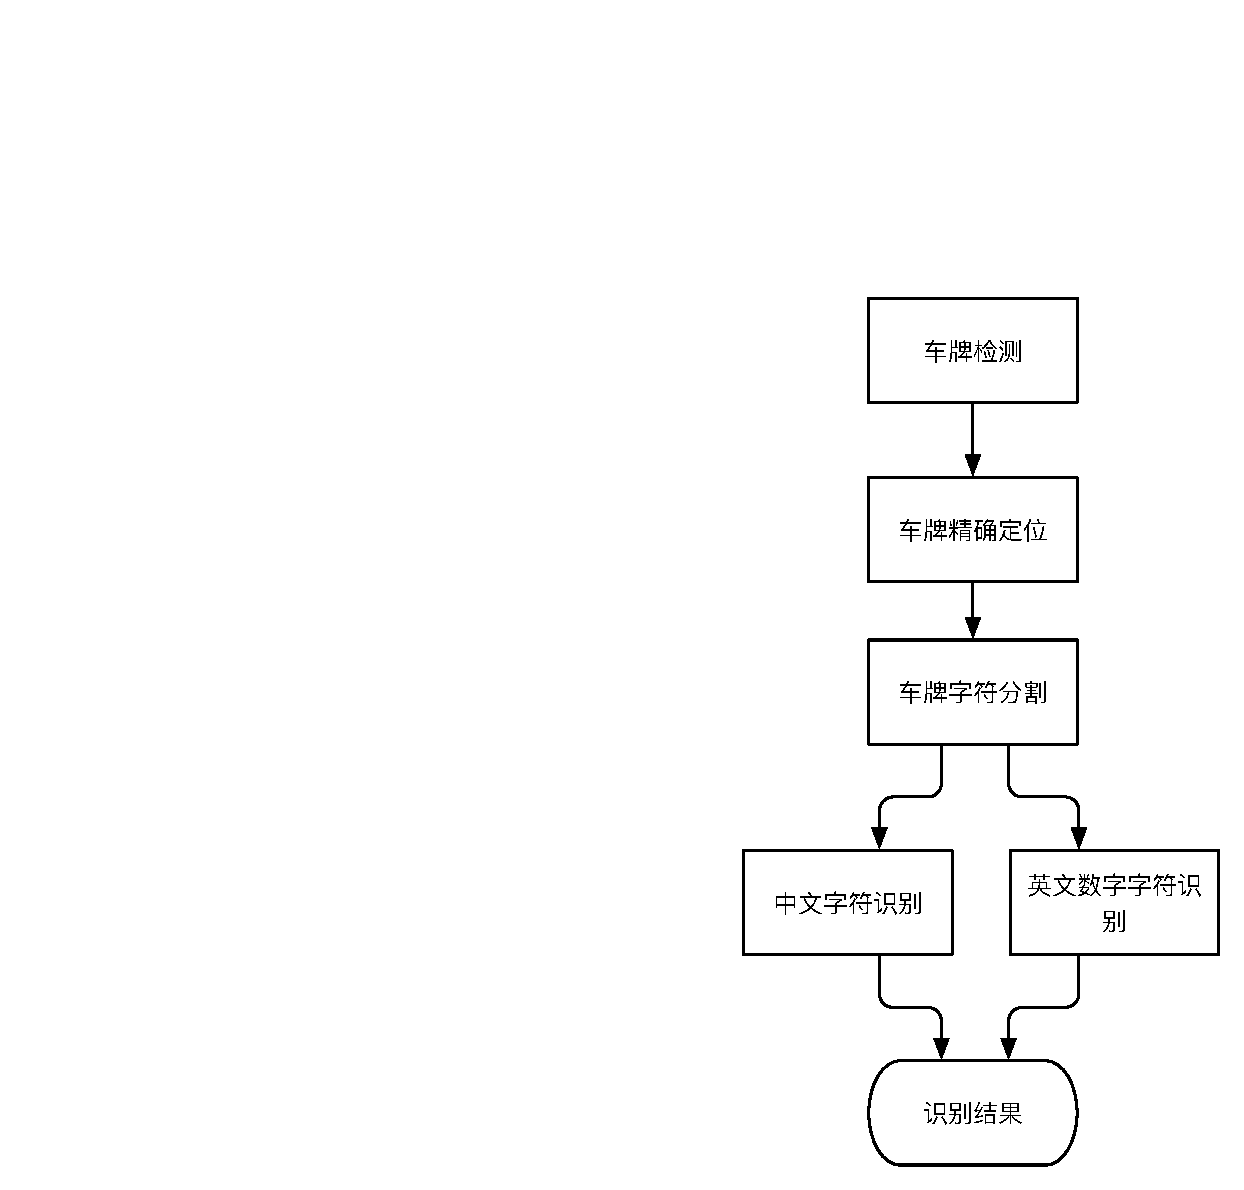
\includegraphics[height=0.8\textheight]{./Figure/SystemArch.eps}
  \end{figure}
\end{frame}

\part{车牌检测}

\section{传统方法}

\begin{frame}
  \frametitle{常见的传统方法}
  \begin{itemize}
    \item 基于车牌形状的方法
    \item 基于颜色划分的方法
    \item 基于纹理特征的方法
  \end{itemize}
\end{frame}

\begin{frame}
  \frametitle{传统方法的优缺点}
  
  \textcolor{red}{\paragraph{优点}}
  \begin{itemize}
    \item 算法简单,易于实现
    \item 执行速度快
  \end{itemize} 

  \textcolor{red}{\paragraph{缺点}}
  \begin{itemize}
    \item 鲁棒性差
    \item 特殊情况多
    \item 难以适应复杂场合
  \end{itemize}
\end{frame}

\section{Faster R-CNN}

\begin{frame}
  \frametitle{Faster R-CNN简介}
  Faster R-CNN全称Faster Region-Convolution Nerual Network,是由微软亚洲研究院
  Shaoqing Ren\cite{Ren:2015ug}等人在Fast R-CNN\cite{Girshick:2015ib}及其前身
  R-CNN\cite{Girshick:2014jx}的基础上提出的一种通用目标检测算法。
  
  \textcolor{red}{\paragraph{优点}}
  \begin{itemize}
    \item 是目前准确率最高的目标检测算法之一
    \item 性能优异,能达到准实时级的检测速度
  \end{itemize} 

  \textcolor{red}{\paragraph{缺点}}
  \begin{itemize}
    \item 需要大量标注过的训练数据
    \item 需要使用GPU加速
  \end{itemize}
\end{frame}

\begin{frame}
  \frametitle{Faster R-CNN原理}
  
  \begin{figure}[ht]
    \centering
    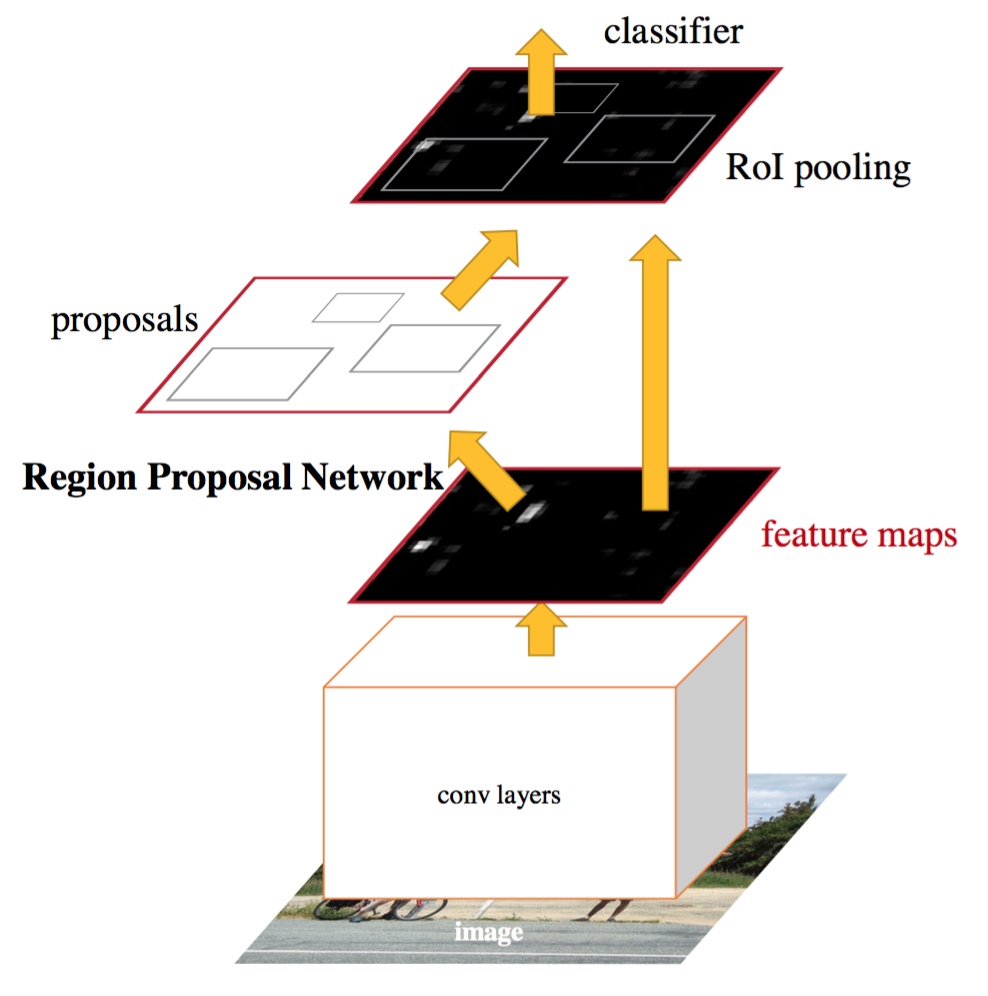
\includegraphics[height=0.8\textheight]{./Figure/FasterRCNN.png}
    \caption{Faster R-CNN结构图}\label{Fig:FasterRCNN}
  \end{figure}
\end{frame}

\section{效果展示}

\begin{frame}
  \frametitle{效果展示}
  \begin{figure}[th]
    \centering
    \subcaptionbox{示例一}
    {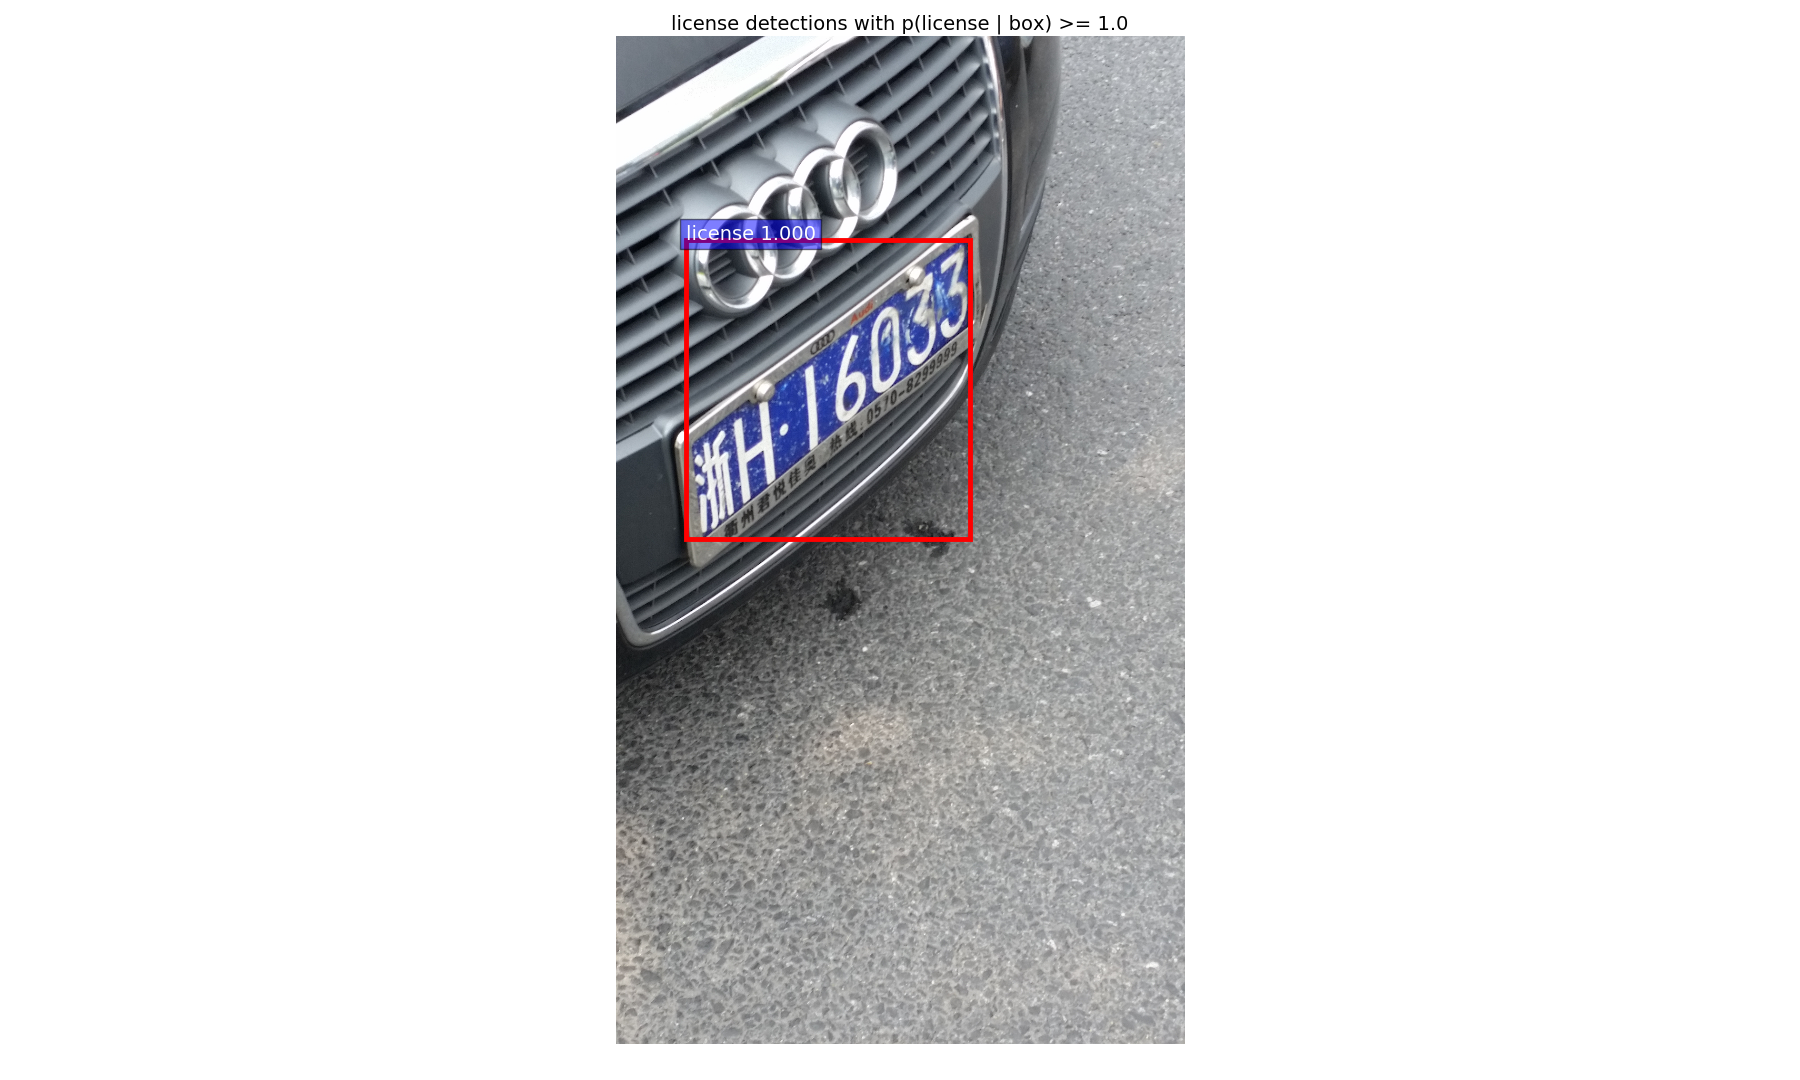
\includegraphics[height=0.6\textheight, keepaspectratio]{./Figure/DetectionDemo.png}}
    \subcaptionbox{示例二}
    {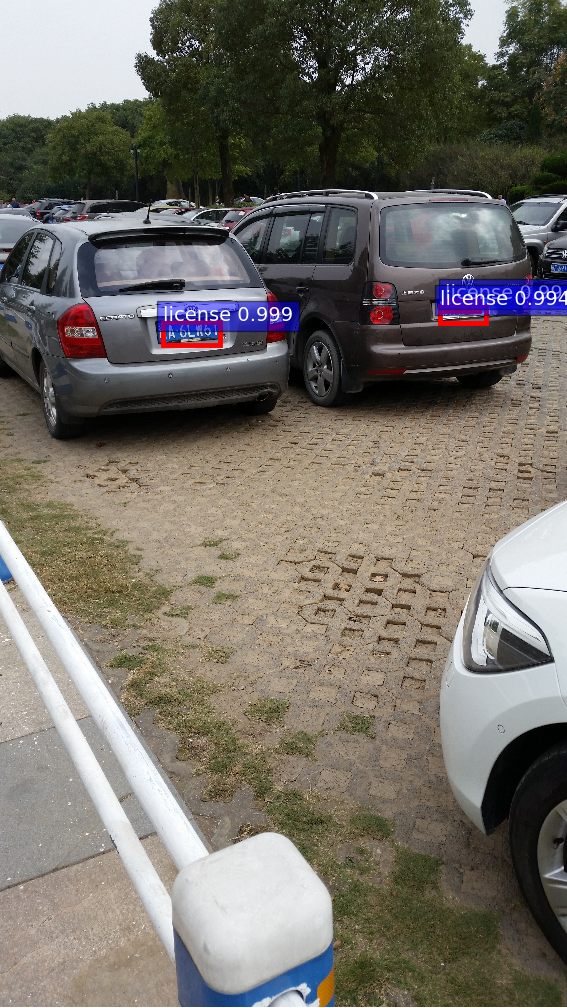
\includegraphics[height=0.6\textheight, keepaspectratio]{./Figure/DetectionDemo2.png}}
    \caption{使用Faster R-CNN进行车牌检测}\label{Fig:DetectionDemo}
  \end{figure}
\end{frame}

\part{车牌定位}

\section{传统方法}

\begin{frame}
  \frametitle{常见的传统方法}

  \begin{itemize}
    \item 基于边缘检测的定位方法
    \item 基于形态学的定位方法
    \item 基于颜色划分的定位方法
  \end{itemize}
\end{frame}

\begin{frame}
  \frametitle{传统方法的优缺点}

  \textcolor{red}{优点}
  \begin{itemize}
    \item 简单,容易实现,速度快
  \end{itemize}

  \textcolor{red}{缺点}
  \begin{itemize}
    \item 难以处理的特殊情况多,鲁棒性不强
    \item 抗仿射、投影变换的能力差
  \end{itemize}
\end{frame}

\section{使用CNN进行车牌定位}

\begin{frame}
  \frametitle{使用CNN进行车牌定位}

  我们可以仿照Faster R-CNN的思路,使用CNN对车牌的四个顶点(关键点)坐标进行回归,
  以实现车牌定位,这种方法的优缺点如下:

  \textcolor{red}{优点}
  \begin{itemize}
    \item 鲁棒性强
  \end{itemize}

  \textcolor{red}{缺点}
  \begin{itemize}
    \item 效果受数据影响大,需要大量标注过的训练数据
    \item CNN抗旋转的能力差,因此需要做数据扩充
    \item 和车牌检测任务有所重复,可进行合并
  \end{itemize}
\end{frame}

\section{效果展示}

\begin{frame}
  \frametitle{效果展示}

  \begin{figure}[ht]
    \centering
    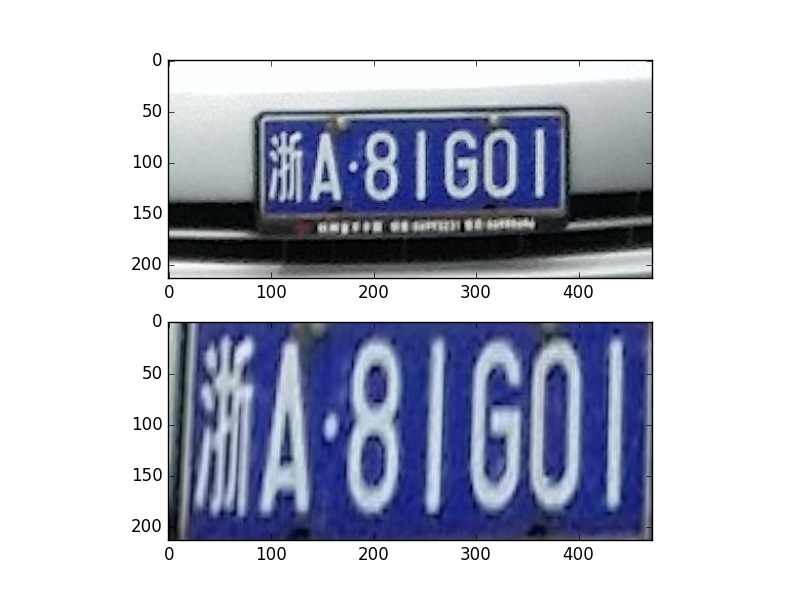
\includegraphics[width=1.0\linewidth]{./Figure/LocalizationDemo.png}
    \caption{车牌定位效果图}\label{Fig:LocalizationDemo}
  \end{figure}
\end{frame}

\part{字符分割}

\section{传统方法}

\begin{frame}
  \frametitle{常见的传统方法}
  
  \begin{itemize}
    \item 基于直方图投影的分割方法
    \item 基于连通域分析的分割方法
  \end{itemize}
\end{frame}

\begin{frame}
  \frametitle{传统方法的优缺点}

  \textcolor{red}{优点}
  \begin{itemize}
    \item 简单,容易实现,速度快
  \end{itemize}

  \textcolor{red}{缺点}
  \begin{itemize}
    \item 基于直方图投影的分割方法要求车牌水平,不能抵抗倾斜等仿射变换
    \item 基于连通域分析的分割方法效果依赖于车牌二值化的效果,因此对图像质量要求
      高,鲁棒性差
  \end{itemize}
\end{frame}

\section{基于Class-specific Extremal Region的分割方法}

\begin{frame}
  \frametitle{Extremal Region的定义}
  \begin{definition}
    我们首先定义图像的一个Region为图像的一个连续子区域。这里的连续是指,该区域中
    像素点总满足某种邻接关系(本文中均指4-邻接,即一个像素和它的上下左右四个像素
    邻接,除此之外还有8-邻接关系)。
  \end{definition}

  \begin{definition}
    我们说一个Region为一个Extremal Region,是指该Region的边界像素值比内部像素值
    高出许多。
  \end{definition}

  \begin{block}{备注}
    以上定义仅做说明用途,详细的数学定义请参考论文4.1.1节
  \end{block}
\end{frame}

\begin{frame}
  \frametitle{Class-specific Extremal Region简介}
  
  Neumann等人于2012年提出了一种\cite{Neumann:2012ik}名为Class-specific
  Extremal Region(CSER)的方法并成功应用于自然场景中的字符检测与定位问题。

  该方法的核心思想是使用两个级联AdaBoost分类器对ER进行筛选,从而快速准确地提取图
  像中的字符区域。

  该方法最终成功在ICDAR Robust Reading竞赛中成功夺取桂冠,充分证明了其有效性。
\end{frame}

\begin{frame}
  \frametitle{使用CSER进行文字检测}
  
  CSER使用两个级联的AdaBoost分类器对产生的ER候选区域进行筛选:

  \begin{itemize}
  \item 第一级分类器使用少而高效的特征进行粗筛选。
  \item 第二级分类器在第一级分类器特征的基础上,使用一些更为有效的特征进行进一步筛选。
  \end{itemize}
  
  \begin{block}{备注}
    由于两个分类器使用的特征定义稍显复杂,在此不再赘述,详情请参考论文4.1.2节
  \end{block}
\end{frame}

\begin{frame}
  \frametitle{使用CSER进行车牌字符分割}
  
  为了进一步去除,假阳性的ER区域,我们在此使用一些车牌的结构信息进行进一步筛选,
  如:
  
  \begin{itemize}
    \item ER相对尺寸
    \item ER长宽比
    \item ER相对位置关系
    \item 其他筛选标准……
  \end{itemize}

  通过上述方法首先得到6个英文、数字字符区域。

  然后以此来推断车牌中中文字符的区域。

  最终便得出所有的车牌字符区域。
\end{frame}

\section{效果展示}

\begin{frame}
  \frametitle{使用CSER产生候选区域}
  
  \begin{figure}[ht]
    \centering
    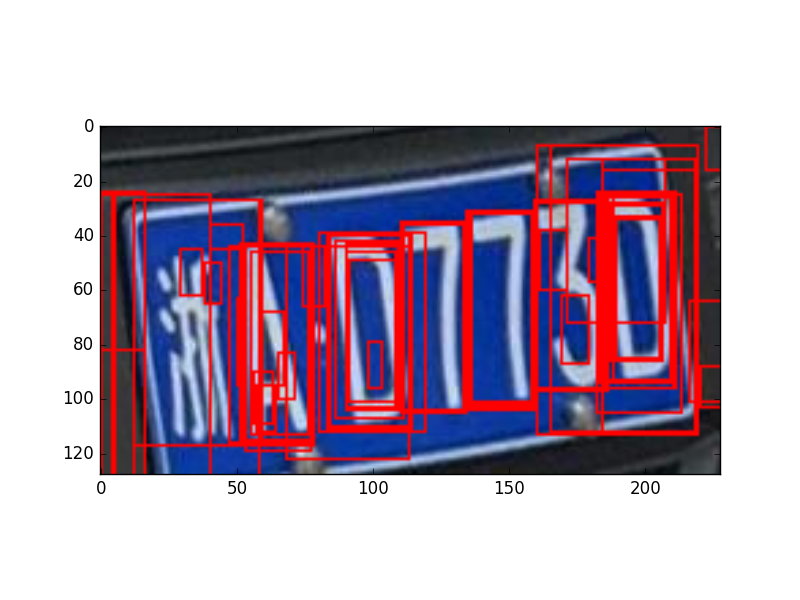
\includegraphics[height=0.6\textheight]{./Figure/AllERs.png}
    \caption{使用CSER提取出的所有候选区}\label{Fig:AllERs}
  \end{figure}
\end{frame}

\begin{frame}
  \frametitle{最终效果}
  
  \begin{figure}[th]
    \centering
    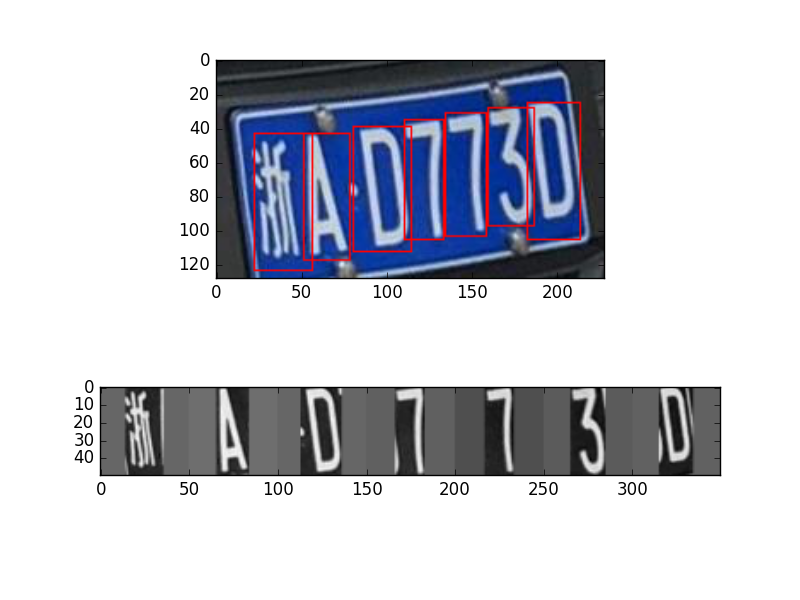
\includegraphics[height=0.6\textheight, keepaspectratio]{./Figure/SegmentationDemo.png}
    \caption{车牌字符分割效果展示}\label{Fig:SegmentationDemo}
  \end{figure}
\end{frame}

\part{字符识别}

\section{使用CNN进行字符识别}

\begin{frame}
  \frametitle{使用CNN进行字符识别}

  \begin{figure}[ht]
    \centering
    \subcaptionbox{中文}
    {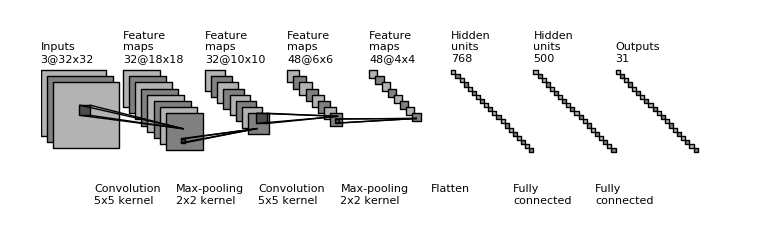
\includegraphics[height=0.25\textheight, keepaspectratio]{./Figure/RecognitionChinese.png}}
    \subcaptionbox{英文及数字}
    {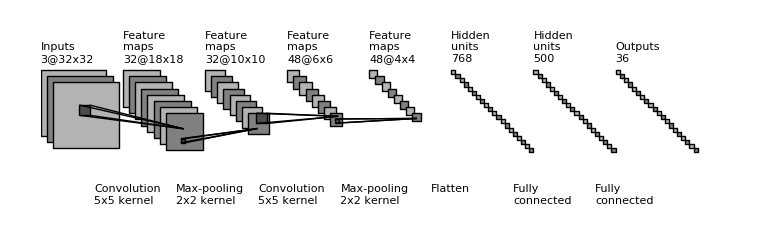
\includegraphics[height=0.25\textheight, keepaspectratio]{./Figure/RecognitionAlnum.png}}
    \caption{字符识别CNN模型} \label{Fig:RecognitionCNN}
  \end{figure}
\end{frame}

\begin{frame}
  \frametitle{效果展示}

  \begin{figure}[ht]
    \centering
    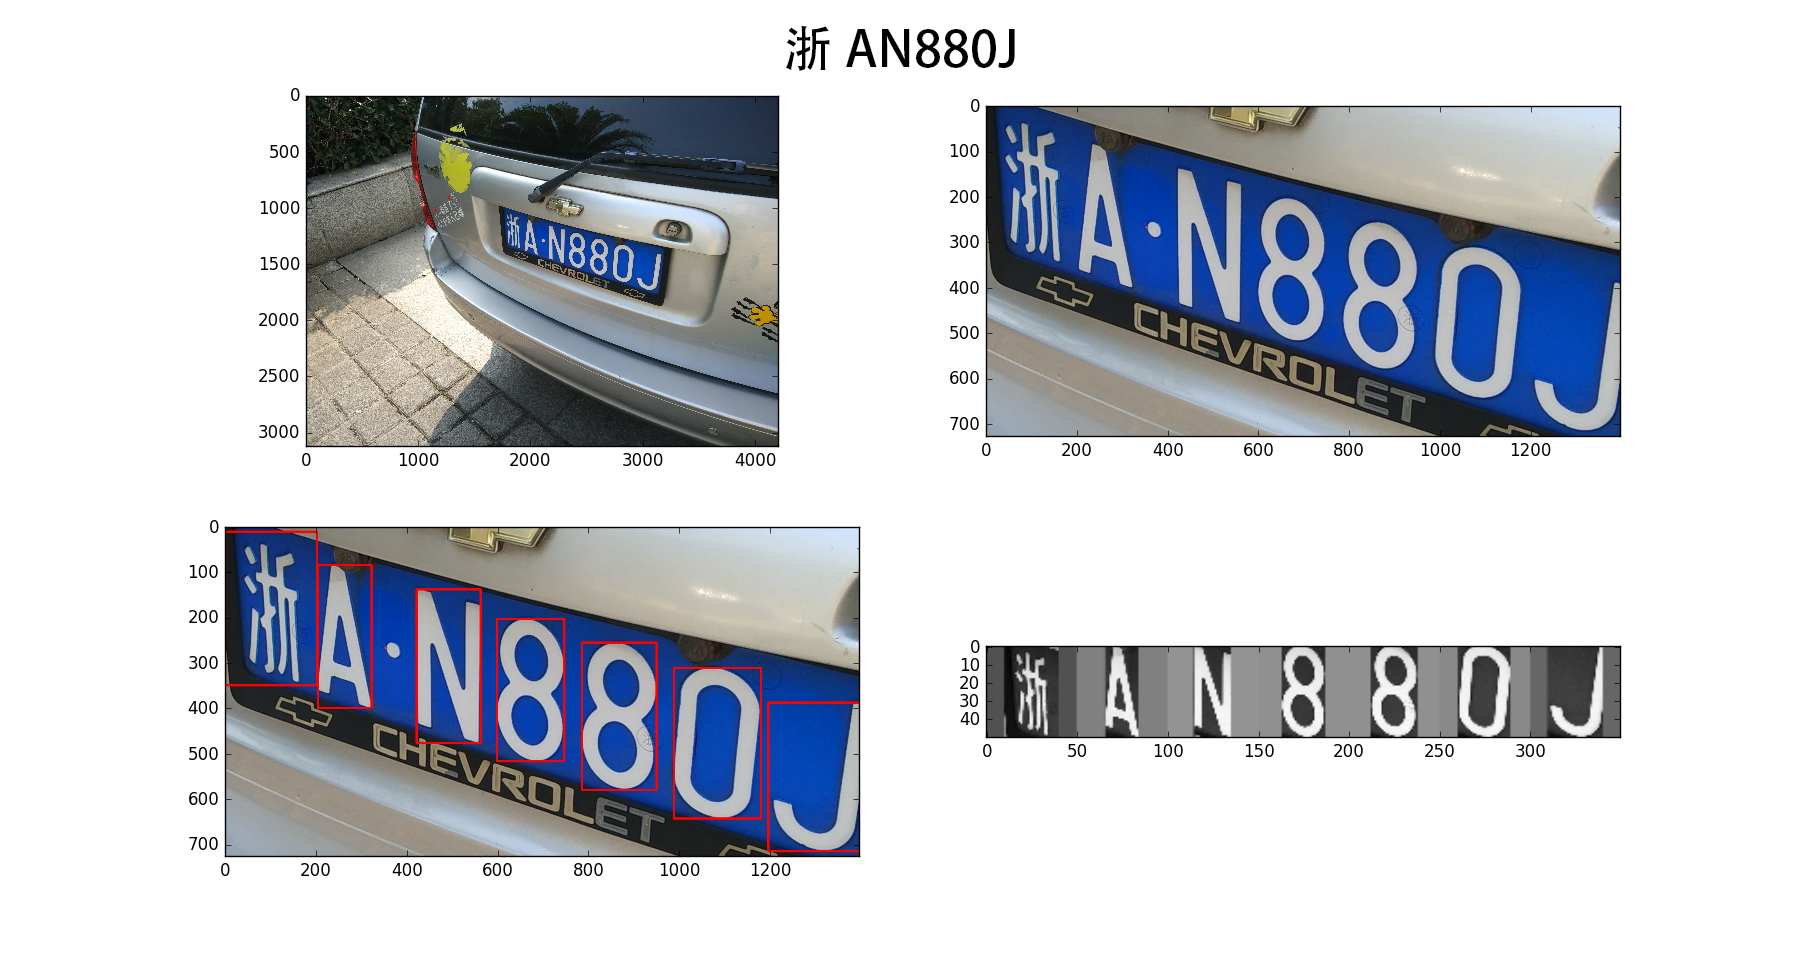
\includegraphics[width=1.0\linewidth]{./Figure/End2EndDemo2.png}
    \caption{系统运行效果}\label{Fig:End2EndDemo}
  \end{figure}
\end{frame}

\part{总结与展望}

\section{总结}

\begin{frame}
  \frametitle{总结}

  可以看到,基于深度学习的车牌识别系统有着鲁棒性强、人工干预少、可定制性强等传统
  方法无法比拟的优点,有着广阔的前景。
\end{frame}

\section{展望}

\begin{frame}
  \frametitle{展望}

  但是我们的系统也有许多可以改进的地方:
  \begin{itemize}
    \item 使用YOLO\cite{Redmon:2015tl}、SSD\cite{Liu:2015wa}等速度更快的算法替代Faster R-CNN进行车牌检测
    \item 将车牌定位整合进车牌检测中
    \item 使用CUDA实现CSER方法以提升性能
    \item 在字符分割任务中使用非极大抑制剔除冗余的ER区域
    \item 等等
    \end{itemize}
  这些都有待进一步的研究、实验以进行验证。
\end{frame}    

\part{参考文献}

\begin{frame}[t, allowframebreaks]
  \frametitle{参考文献}
  \printbibliography
\end{frame}

{ \xdbg
\begin{frame}[plain, noframenumbering]
  \finalpage{{\huge 感谢各位评委老师的观看!}}
\end{frame}
}

\end{document}